% Brief expl
This appendix reports all graphs and tables related to the reading experiments conducted. Results are reported first expressed as latency (measured during the experiments) and then as throughput (computed from the latency and table size).


%%%%%%%%%%%%%%%%%%%%%%%%%%%%%%%%%%%%%%%%%%%%%%%%%%%%%%%%%%%%%%%%%
%%%%%%%%%%%%              LATENCY             %%%%%%%%%%%%%%%%%%%
%%%%%%%%%%%%%%%%%%%%%%%%%%%%%%%%%%%%%%%%%%%%%%%%%%%%%%%%%%%%%%%%%
\begin{figure}
    \centering
    \begin{minipage}[b]{\textwidth}
        \centering
        \captionof{table}[Read experiment - Latency - 1 CPU core]{Read experiment results expressed as latency. The experiment was performed with one \glstext{CPU} core.}
        \label{tbl:appx_res_read_time_1_core}
        \begin{tabular}{c r S[table-format=5.5] S[table-format=5.5] S[table-format=5.5]} 
            \toprule
            \multirow{2}{*}{{Pipeline\Tstrut\Bstrut}} & \multirow{2}{*}{{\thead{Number\\ of rows}}} & {\multirow{2}{*}{{\thead{Latency \\ (seconds)}}}} & \multicolumn{2}{c}{{\thead{Latency (seconds) \\95\% Confidence Interval}}}\\
                                                      &                                             &                                                   & {low} & {high}\\
            \midrule
            \multirow{5}{4em}{delta-rs\\ HopsFS} & 10K  &    0.05342 &    0.03916 &    0.08112\\ 
                                                 & 100K &    0.05757 &    0.05518 &    0.06046\\ 
                                                 & 1M   &    0.53855 &    0.52558 &    0.55229\\
                                                 & 6M   &    1.94899 &    1.93007 &    1.96860\\
                                                 & 60M  &   22.98065 &   22.84067 &   23.14206\\
            \midrule
            \multirow{5}{4em}{delta-rs\\ LocalFS} & 10K  &    0.00419 &    0.00268 &    0.00644\\ 
                                                  & 100K &    0.02696 &    0.01966 &    0.03433\\ 
                                                  & 1M   &    0.42009 &    0.40613 &    0.43563\\
                                                  & 6M   &    1.68223 &    1.65981 &    1.70440\\
                                                  & 60M  &   19.56547 &   19.34690 &   19.77724\\
            \midrule
            \multirow{5}{4em}{Legacy} & 10K  &     0.63159 &    0.62414 &    0.64157\\ 
                                      & 100K &     2.65010 &    2.64272 &    2.65876\\ 
                                      & 1M   &     8.59636 &    8.34094 &    8.90047\\
                                      & 6M   &    33.52964 &   33.23886 &   33.86591\\
                                      & 60M  &    33.69772 &   33.36262 &   34.08665\\
            \bottomrule
        \end{tabular}
    \end{minipage}
    \begin{minipage}[b]{\textwidth}
        \centering
        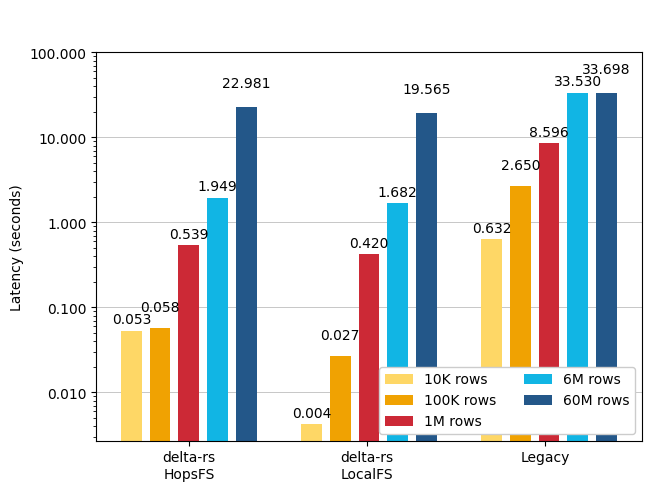
\includegraphics[width=\textwidth]{figures/99-appendix/results-diagrams/read/read_time_1_core.png}
        \caption[Histogram of the read experiment - Latency - 1 CPU core]{Histogram in log-scale of the read experiment results expressed as latency. The experiment was performed with one \glstext{CPU} core.}
        \label{fig:appx_res_read_time_1_core}
    \end{minipage}
\end{figure}

\begin{figure}
    \centering
    \begin{minipage}[b]{\textwidth}
        \centering
        \captionof{table}[Read experiment - Latency - 2 CPU cores]{Read experiment results expressed as latency. The experiment was performed with two \glstext{CPU} cores.}
        \label{tbl:appx_res_read_time_2_cores}
        \begin{tabular}{c r S[table-format=5.5] S[table-format=5.5] S[table-format=5.5]} 
            \toprule
            \multirow{2}{*}{{Pipeline\Tstrut\Bstrut}} & \multirow{2}{*}{{\thead{Number\\ of rows}}} & {\multirow{2}{*}{{\thead{Latency \\ (seconds)}}}} & \multicolumn{2}{c}{{\thead{Latency (seconds) \\95\% Confidence Interval}}}\\
                                                      &                                             &                                                   & {low} & {high}\\
            \midrule
            \multirow{5}{4em}{delta-rs\\ HopsFS} & 10K  &    0.04132 &    0.03933 &    0.04378\\ 
                                                 & 100K &    0.05690 &    0.05123 &    0.06693\\ 
                                                 & 1M   &    0.23413 &    0.22528 &    0.24426\\
                                                 & 6M   &    0.90832 &    0.89967 &    0.91744\\
                                                 & 60M  &   11.41325 &   11.27661 &   11.58899\\
            \midrule
            \multirow{5}{4em}{delta-rs\\ LocalFS} & 10K  &    0.00287 &    0.00278 &    0.00299\\ 
                                                  & 100K &    0.01306 &    0.01041 &    0.01610\\ 
                                                  & 1M   &    0.19977 &    0.18858 &    0.21056\\
                                                  & 6M   &    0.74764 &    0.73503 &    0.76013\\
                                                  & 60M  &    9.44693 &    9.37207 &    9.51753\\
            \midrule
            \multirow{5}{4em}{Legacy} & 10K  &     0.62492 &    0.62210 &    0.62822\\ 
                                      & 100K &     2.66339 &    2.65616 &    2.67166\\ 
                                      & 1M   &     8.61667 &    8.30989 &    8.94938\\
                                      & 6M   &    33.37519 &   33.09688 &   33.67065\\
                                      & 60M  &    33.64281 &   33.30150 &   34.06307\\
            \bottomrule
        \end{tabular}
    \end{minipage}
    \begin{minipage}[b]{\textwidth}
        \centering
        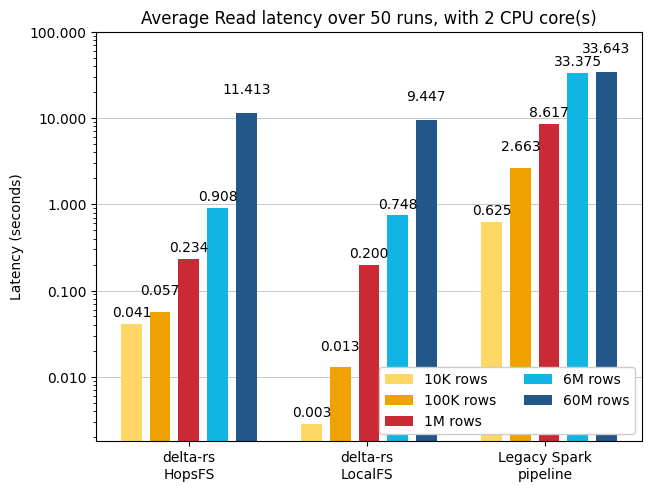
\includegraphics[width=\textwidth]{figures/99-appendix/results-diagrams/read/read_time_2_core.png}
        \caption[Histogram of the read experiment - Latency - 2 CPU cores]{Histogram in log-scale of the read experiment results expressed as latency. The experiment was performed with two \glstext{CPU} cores.}
        \label{fig:appx_res_read_time_2_cores}
    \end{minipage}
\end{figure}

\begin{figure}
    \centering
    \begin{minipage}[b]{\textwidth}
        \centering
        \captionof{table}[Read experiment - Latency - 4 CPU cores]{Read experiment results expressed as latency. The experiment was performed with four \glstext{CPU} cores.}
        \label{tbl:appx_res_read_time_4_cores}
        \begin{tabular}{c r S[table-format=5.5] S[table-format=5.5] S[table-format=5.5]} 
            \toprule
            \multirow{2}{*}{{Pipeline\Tstrut\Bstrut}} & \multirow{2}{*}{{\thead{Number\\ of rows}}} & {\multirow{2}{*}{{\thead{Latency \\ (seconds)}}}} & \multicolumn{2}{c}{{\thead{Latency (seconds) \\95\% Confidence Interval}}}\\
                                                      &                                             &                                                   & {low} & {high}\\
            \midrule
            \multirow{5}{4em}{delta-rs\\ HopsFS} & 10K  &    0.04336 &    0.03922 &   0.05092\\ 
                                                 & 100K &    0.05540 &    0.05378 &   0.05789\\ 
                                                 & 1M   &    0.18847 &    0.15157 &   0.25189\\
                                                 & 6M   &    0.53124 &    0.50778 &   0.57105\\
                                                 & 60M  &    5.58011 &    5.54397 &   5.61936\\
            \midrule
            \multirow{5}{4em}{delta-rs\\ LocalFS} & 10K  &    0.00268 &   0.00259 &   0.00279\\ 
                                                  & 100K &    0.00923 &   0.00852 &   0.01020\\ 
                                                  & 1M   &    0.08971 &   0.08388 &   0.09503\\
                                                  & 6M   &    0.37021 &   0.36018 &   0.38032\\
                                                  & 60M  &    4.81023 &   4.79338 &   4.82789\\
            \midrule
            \multirow{5}{4em}{Legacy} & 10K  &     0.63583 &    0.62352 &    0.65908\\ 
                                      & 100K &     2.63985 &    2.63349 &    2.64623\\ 
                                      & 1M   &     8.75238 &    8.50725 &    9.01383\\
                                      & 6M   &    33.45286 &   33.19461 &   33.75646\\
                                      & 60M  &    33.65245 &   33.27016 &   34.03900\\
            \bottomrule
        \end{tabular}
    \end{minipage}
    \begin{minipage}[b]{\textwidth}
        \centering
        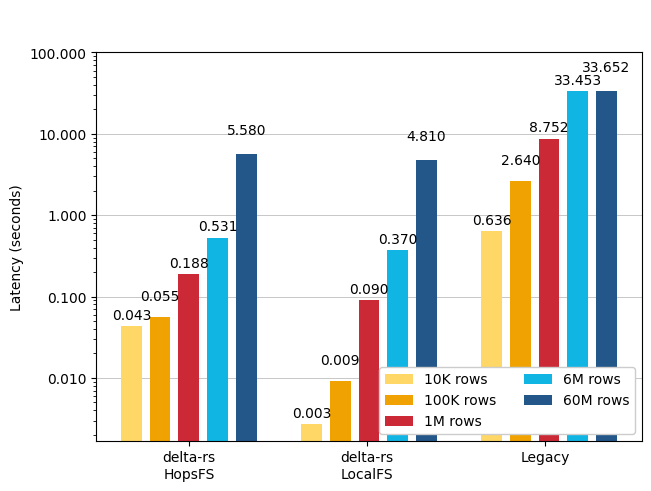
\includegraphics[width=\textwidth]{figures/99-appendix/results-diagrams/read/read_time_4_core.png}
        \caption[Histogram of the read experiment - Latency - 4 CPU cores]{Histogram in log-scale of the read experiment results expressed as latency. The experiment was performed with four \glstext{CPU} cores.}
        \label{fig:appx_res_read_time_4_cores}
    \end{minipage}
\end{figure}

\begin{figure}
    \centering
    \begin{minipage}[b]{\textwidth}
        \centering
        \captionof{table}[Read experiment - Latency - 8 CPU cores]{Read experiment results expressed as latency. The experiment was performed with eight \glstext{CPU} cores.}
        \label{tbl:appx_res_read_time_8_cores}
        \begin{tabular}{c r S[table-format=5.5] S[table-format=5.5] S[table-format=5.5]} 
            \toprule
            \multirow{2}{*}{{Pipeline\Tstrut\Bstrut}} & \multirow{2}{*}{{\thead{Number\\ of rows}}} & {\multirow{2}{*}{{\thead{Latency \\ (seconds)}}}} & \multicolumn{2}{c}{{\thead{Latency (seconds) \\95\% Confidence Interval}}}\\
                                                      &                                             &                                                   & {low} & {high}\\
            \midrule
            \multirow{5}{4em}{delta-rs\\ HopsFS} & 10K  &    0.04330 &    0.03885 &    0.05119\\ 
                                                 & 100K &    0.05458 &    0.05286 &    0.05663\\ 
                                                 & 1M   &    0.17390 &    0.16992 &    0.17808\\
                                                 & 6M   &    0.49729 &    0.48655 &    0.51019\\
                                                 & 60M  &    2.94236 &    2.85554 &    3.06360\\
            \midrule
            \multirow{5}{4em}{delta-rs\\ LocalFS} & 10K  &    0.00294 &    0.00284 &    0.00307\\ 
                                                  & 100K &    0.00948 &    0.00872 &    0.01056\\ 
                                                  & 1M   &    0.04308 &    0.03934 &    0.04830\\
                                                  & 6M   &    0.17548 &    0.17009 &    0.18080\\
                                                  & 60M  &    2.28550 &    2.27501 &    2.29607\\
            \midrule
            \multirow{5}{4em}{Legacy} & 10K  &     0.62739 &    0.62245 &    0.63259\\ 
                                      & 100K &     2.66217 &    2.65309 &    2.67218\\ 
                                      & 1M   &     8.34757 &    8.13471 &    8.60942\\
                                      & 6M   &    33.42815 &   33.15376 &   33.74947\\
                                      & 60M  &    33.14341 &   32.88303 &   33.41299\\
            \bottomrule
        \end{tabular}
    \end{minipage}
    \begin{minipage}[b]{\textwidth}
        \centering
        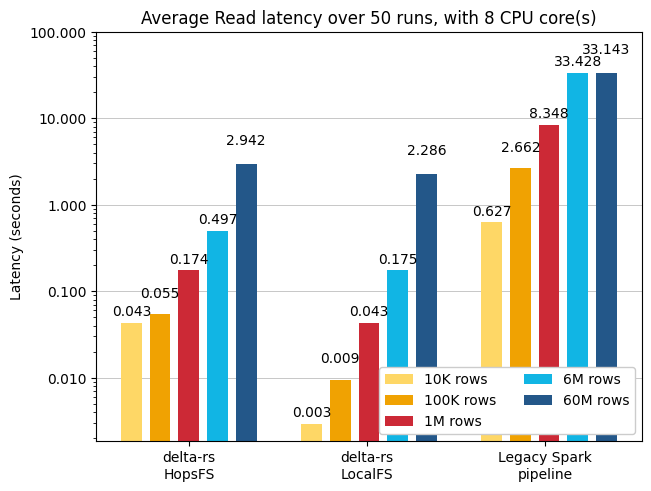
\includegraphics[width=\textwidth]{figures/99-appendix/results-diagrams/read/read_time_8_core.png}
        \caption[Histogram of the read experiment - Latency - 8 CPU cores]{Histogram in log-scale of the read experiment results expressed as latency. The experiment was performed with eight \glstext{CPU} cores.}
        \label{fig:appx_res_read_time_8_cores}
    \end{minipage}
\end{figure}

%%%%%%%%%%%%%%%%%%%%%%%%%%%%%%%%%%%%%%%%%%%%%%%%%%%%%%%%%%%%%%%%%
%%%%%%%%%%%%             THROUGHPUT           %%%%%%%%%%%%%%%%%%%
%%%%%%%%%%%%%%%%%%%%%%%%%%%%%%%%%%%%%%%%%%%%%%%%%%%%%%%%%%%%%%%%%

\begin{figure}
    \centering
    \begin{minipage}[b]{\textwidth}
        \centering
        \captionof{table}[Read experiment - Throughput - 1 CPU core]{Read experiment results expressed as throughput. The experiment was performed with one \glstext{CPU} core.}
        \label{tbl:appx_res_read_throughput_1_core}
        \begin{tabular}{c r S[table-format=5.5] S[table-format=5.5] S[table-format=5.5]} 
            \toprule
            \multirow{2}{*}{{Pipeline\Tstrut\Bstrut}} & \multirow{2}{*}{{\thead{Number\\ of rows}}} & {\multirow{2}{*}{{\thead{Throughput \\ (k rows/second)}}}} & \multicolumn{2}{c}{{\thead{Throughput (k rows/second) \\95\% Confidence Interval}}}\\
                                                      &                                             &                                                          & {low} & {high}\\
            \midrule
            \multirow{5}{4em}{delta-rs\\ HopsFS} & 10K  &  187.16853 &  123.26555 &  255.36173\\ 
                                                 & 100K & 1736.90799 & 1653.91940 & 1811.92857\\ 
                                                 & 1M   & 1856.83167 & 1810.61318 & 1902.65361\\
                                                 & 6M   & 3078.51299 & 3047.83914 & 3108.69431\\
                                                 & 60M  & 2610.89146 & 2592.68185 & 2626.89240\\
            \midrule
            \multirow{5}{4em}{delta-rs\\ LocalFS} & 10K  & 2384.58699 & 1552.08552 & 3721.36068\\ 
                                                  & 100K & 3708.25787 & 2912.43600 & 5084.75715\\ 
                                                  & 1M   & 2380.40381 & 2295.50154 & 2462.25814\\
                                                  & 6M   & 3566.67454 & 3520.29796 & 3614.87006\\
                                                  & 60M  & 3066.62644 & 3033.78996 & 3101.27165\\
            \midrule
            \multirow{5}{4em}{Legacy} & 10K  &    15.83285 &   15.58654 &   16.02196\\ 
                                      & 100K &    37.73432 &   37.61140 &   37.83975\\ 
                                      & 1M   &   116.32820 &  112.35350 &  119.89044\\
                                      & 6M   &   178.94612 &  177.16928 &  180.51159\\
                                      & 60M  &  1780.53563 & 1760.21974 & 1798.41962\\
            \bottomrule
        \end{tabular}
    \end{minipage}
    \begin{minipage}[b]{\textwidth}
        \centering
        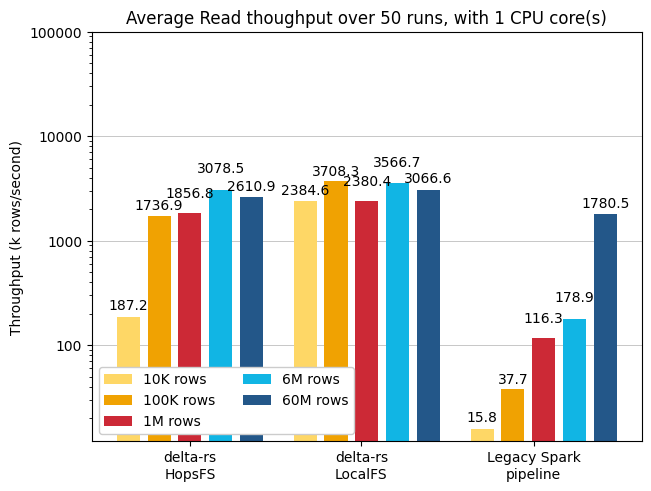
\includegraphics[width=\textwidth]{figures/99-appendix/results-diagrams/read/read_throughput_1_core.png}
        \caption[Histogram of the read experiment - Throughput - 1 CPU core]{Histogram in log-scale of the read experiment results expressed as throughput. The experiment was performed with one \glstext{CPU} core.}
        \label{fig:appx_res_read_throughput_1_core}
    \end{minipage}
\end{figure}

\begin{figure}
    \centering
    \begin{minipage}[b]{\textwidth}
        \centering
        \captionof{table}[Read experiment - Throughput - 2 CPU cores]{Read experiment results expressed as throughput. The experiment was performed with two \glstext{CPU} cores.}
        \label{tbl:appx_res_read_throughput_2_cores}
        \begin{tabular}{c r S[table-format=5.5] S[table-format=5.5] S[table-format=5.5]} 
            \toprule
            \multirow{2}{*}{{Pipeline\Tstrut\Bstrut}} & \multirow{2}{*}{{\thead{Number\\ of rows}}} & {\multirow{2}{*}{{\thead{Throughput \\ (k rows/second)}}}} & \multicolumn{2}{c}{{\thead{Throughput (k rows/second) \\95\% Confidence Interval}}}\\
                                                      &                                             &                                                          & {low} & {high}\\
            \midrule
            \multirow{5}{4em}{delta-rs\\ HopsFS} & 10K  &  241.97833 &  228.37018 &  254.22419\\ 
                                                 & 100K & 1757.17930 & 1494.01876 & 1951.81229\\ 
                                                 & 1M   & 4271.12139 & 4093.98917 & 4438.84612\\
                                                 & 6M   & 6605.54323 & 6539.93631 & 6669.08756\\
                                                 & 60M  & 5257.04658 & 5177.32395 & 5320.74334\\
            \midrule
            \multirow{5}{4em}{delta-rs\\ LocalFS} & 10K  & 3479.95285 & 3339.11982 & 3592.42255\\ 
                                                  & 100K & 7652.74709 & 6210.29638 & 9604.33293\\ 
                                                  & 1M   & 5005.61642 & 4749.17943 & 5302.53656\\
                                                  & 6M   & 8025.19634 & 7893.33251 & 8162.84493\\
                                                  & 60M  & 6351.26715 & 6304.15538 & 6401.99467\\
            \midrule
            \multirow{5}{4em}{Legacy} & 10K  &   16.00183 &   15.91773 &   16.07453\\ 
                                      & 100K &   37.54607 &   37.42979 &   37.64822\\ 
                                      & 1M   &  116.05404 &  111.73951 &  120.33848\\
                                      & 6M   &  179.77424 &  178.19671 &  181.28593\\
                                      & 60M  & 1783.44198 & 1761.43830 & 1801.72013\\
            \bottomrule
        \end{tabular}
    \end{minipage}
    \begin{minipage}[b]{\textwidth}
        \centering
        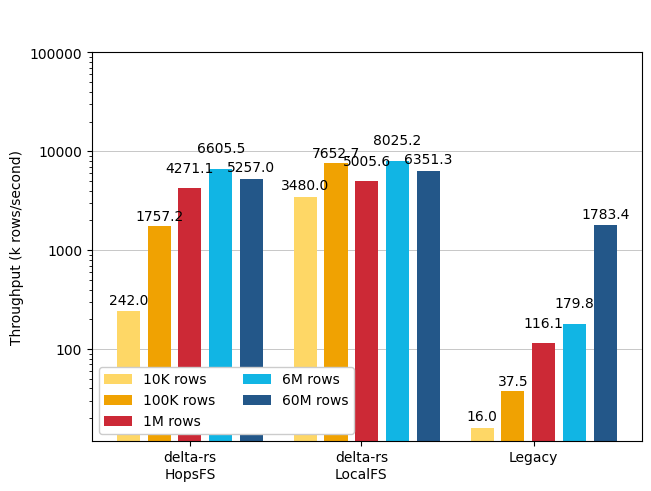
\includegraphics[width=\textwidth]{figures/99-appendix/results-diagrams/read/read_throughput_2_core.png}
        \caption[Histogram of the read experiment - Throughput - 2 CPU cores]{Histogram in log-scale of the read experiment results expressed as throughput. The experiment was performed with two \glstext{CPU} cores.}
        \label{fig:appx_res_read_throughput_2_cores}
    \end{minipage}
\end{figure}

\begin{figure}
    \centering
    \begin{minipage}[b]{\textwidth}
        \centering
        \captionof{table}[Read experiment - Throughput - 4 CPU cores]{Read experiment results expressed as throughput. The experiment was performed with four \glstext{CPU} cores.}
        \label{tbl:appx_res_read_throughput_4_cores}
        \begin{tabular}{c r S[table-format=5.5] S[table-format=5.5] S[table-format=5.5]} 
            \toprule
            \multirow{2}{*}{{Pipeline\Tstrut\Bstrut}} & \multirow{2}{*}{{\thead{Number\\ of rows}}} & {\multirow{2}{*}{{\thead{Throughput \\ (k rows/second)}}}} & \multicolumn{2}{c}{{\thead{Throughput (k rows/second) \\95\% Confidence Interval}}}\\
                                                      &                                             &                                                          & {low} & {high}\\
            \midrule
            \multirow{5}{4em}{delta-rs\\ HopsFS} & 10K  &   230.61925 &   196.37366 &   254.93232\\ 
                                                 & 100K &  1804.73106 &  1727.27256 &  1859.40719\\ 
                                                 & 1M   &  5305.74239 &  3969.95699 &  6597.37404\\
                                                 & 6M   & 11294.12619 & 10506.91939 & 11816.03313\\
                                                 & 60M  & 10752.47511 & 10677.35647 & 10822.55620\\
            \midrule
            \multirow{5}{4em}{delta-rs\\ LocalFS} & 10K  &  3720.94104 &  3572.45085 &  3854.74973\\ 
                                                  & 100K & 10830.88457 &  9802.96062 & 11735.92863\\ 
                                                  & 1M   & 11146.06743 & 10522.54071 & 11921.62257\\
                                                  & 6M   & 16206.97330 & 15775.94387 & 16657.93725\\
                                                  & 60M  & 12473.40492 & 12427.78728 & 12517.25967\\
            \midrule
            \multirow{5}{4em}{Legacy} & 10K  &    15.72724 &   15.17259 &   16.03790\\ 
                                      & 100K &    37.88093 &   37.78959 &   37.97237\\ 
                                      & 1M   &   114.25460 &  110.94061 &  117.54671\\
                                      & 6M   &   179.35680 &  177.74372 &  180.75222\\
                                      & 60M  &  1782.93073 & 1762.68396 & 1803.41764\\
            \bottomrule
        \end{tabular}
    \end{minipage}
    \begin{minipage}[b]{\textwidth}
        \centering
        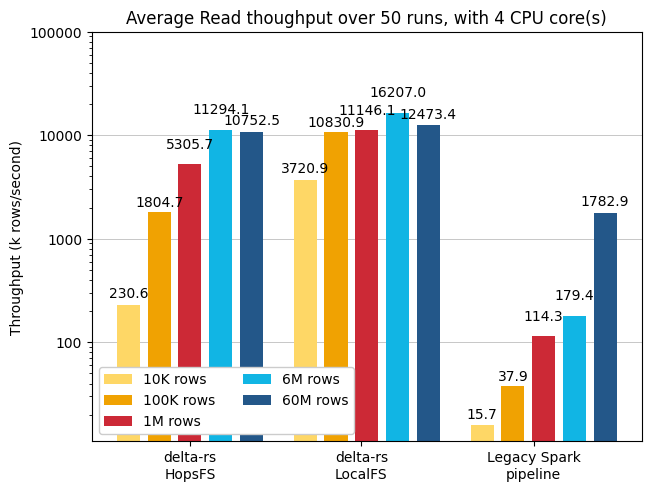
\includegraphics[width=\textwidth]{figures/99-appendix/results-diagrams/read/read_throughput_4_core.png}
        \caption[Histogram of the read experiment - Throughput - 4 CPU cores]{Histogram in log-scale of the read experiment results expressed as throughput. The experiment was performed with four \glstext{CPU} cores.}
        \label{fig:appx_res_read_throughput_4_cores}
    \end{minipage}
\end{figure}

\begin{figure}
    \centering
    \begin{minipage}[b]{\textwidth}
        \centering
        \captionof{table}[Read experiment - Throughput - 8 CPU cores]{Read experiment results expressed as throughput. The experiment was performed with eight \glstext{CPU} cores.}
        \label{tbl:appx_res_read_throughput_8_cores}
        \begin{tabular}{c r S[table-format=5.5] S[table-format=5.5] S[table-format=5.5]} 
            \toprule
            \multirow{2}{*}{{Pipeline\Tstrut\Bstrut}} & \multirow{2}{*}{{\thead{Number\\ of rows}}} & {\multirow{2}{*}{{\thead{Throughput \\ (k rows/second)}}}} & \multicolumn{2}{c}{{\thead{Throughput (k rows/second) \\95\% Confidence Interval}}}\\
                                                      &                                             &                                                          & {low} & {high}\\
            \midrule
            \multirow{5}{4em}{delta-rs\\ HopsFS} & 10K  &   230.92518 &   195.34544 &   257.36067\\ 
                                                 & 100K &  1832.05683 &  1765.75684 &  1891.54456\\ 
                                                 & 1M   &  5750.34366 &  5615.17071 &  5885.01795\\
                                                 & 6M   & 12065.18202 & 11760.17893 & 12331.70977\\
                                                 & 60M  & 20391.77956 & 19584.75363 & 21011.72136\\
            \midrule
            \multirow{5}{4em}{delta-rs\\ LocalFS} & 10K  &  3390.32242 &  3256.07486 &  3510.69231\\ 
                                                  & 100K & 10545.41087 &  9465.27536 & 11463.06073\\ 
                                                  & 1M   & 23212.46679 & 20701.23033 & 25414.13122\\
                                                  & 6M   & 34191.39637 & 33185.18129 & 35275.25456\\
                                                  & 60M  & 26252.42019 & 26131.51836 & 26373.48880\\
            \midrule
            \multirow{5}{4em}{Legacy} & 10K  &    15.93901 &   15.80791 &   16.06539\\ 
                                      & 100K &    37.56330 &   37.42250 &   37.69186\\ 
                                      & 1M   &   119.79520 &  116.15177 &  122.92995\\
                                      & 6M   &   179.48942 &  177.78054 &  180.97490\\
                                      & 60M  &  1810.31436 & 1795.70867 & 1824.64883\\
            \bottomrule
        \end{tabular}
    \end{minipage}
    \begin{minipage}[b]{\textwidth}
        \centering
        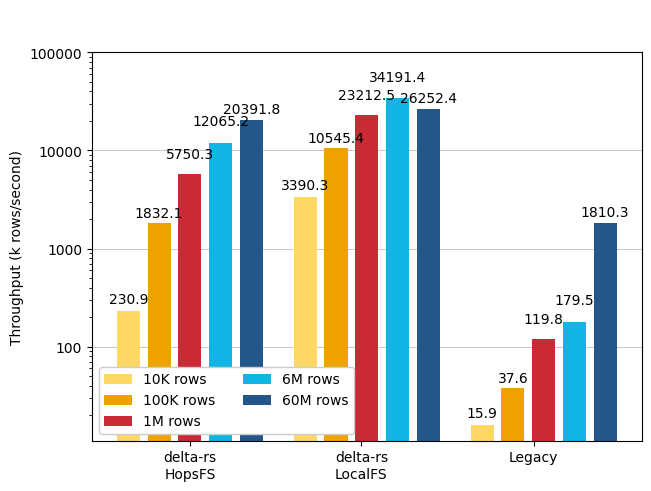
\includegraphics[width=\textwidth]{figures/99-appendix/results-diagrams/read/read_throughput_8_core.png}
        \caption[Histogram of the read experiment - Throughput - 8 CPU cores]{Histogram in log-scale of the read experiment results expressed as throughput. The experiment was performed with eight \glstext{CPU} cores.}
        \label{fig:appx_res_read_throughput_8_cores}
    \end{minipage}
\end{figure}